\section{Auswertung}
\label{sec:Auswertung}
\subsection{Analyse der Filterkurve des Selektiv-Verstärkers}
Die aufgenommenen Messwerte zur Bestimmung der Güte des Selektivverstärkers sind in Tabelle (\ref{tab:Selektivverstärker}) 
aufgelistet.

\begin{table}[H]
  \centering
  \caption{Gemessene Ausgangsspannung $U_{\text{A}}$ des Selektivverstärkers zu verschiedenen Frequenzen $\nu$}
  \label{tab:Selektivverstärker}
  \begin{tblr}{colspec={c c | c c | c c | c c}}
      \toprule
      $\nu \, \left[\unit{\kilo\hertz}\right]$ & $U_{\text{A}} \left[\unit{\volt}\right]$ & $\nu \, \left[\unit{\kilo\hertz}\right]$ & $U_{\text{A}} \left[\unit{\volt}\right]$ & $\nu \, \left[\unit{\kilo\hertz}\right]$ & $U_{\text{A}} \left[\unit{\volt}\right]$ & $\nu \, \left[\unit{\kilo\hertz}\right]$ & $U_{\text{A}} \left[\unit{\volt}\right]$\\
      \midrule
      20,000 & 1,0 & 30,500 & 12,9 & 31,360 & 56,0 & 31,834 & 61,9 \\
      21,000 & 1,1 & 30,600 & 14,3 & 31,402 & 60,0 & 31,857 & 57,1 \\
      22,200 & 1,3 & 30,720 & 16,2 & 31,420 & 63,0 & 31,883 & 52,4 \\
      23,200 & 1,5 & 30,810 & 18,1 & 31,440 & 68,0 & 31,917 & 47,6 \\
      24,100 & 1,7 & 30,900 & 20,5 & 31,460 & 73,0 & 31,951 & 42,9 \\
      25,000 & 2,0 & 31,008 & 24,3 & 31,480 & 78,0 & 31,995 & 38,1 \\
      26,000 & 2,4 & 31,024 & 24,8 & 31,500 & 84,0 & 32,046 & 33,3 \\
      27,000 & 3,0 & 31,046 & 25,7 & 31,520 & 90,0 & 32,122 & 28,6 \\
      28,040 & 4,0 & 31,060 & 26,2 & 31,540 & 95,0 & 32,220 & 23,8 \\
      29,000 & 5,6 & 31,080 & 27,1 & 31,562 & 101,0 & 32,347 & 19,0 \\
      29,120 & 5,9 & 31,107 & 28,6 & 31,580 & 95,2 & 32,625 & 14,3 \\
      29,200 & 6,1 & 31,120 & 30,0 & 31,600 & 104,8 & 33,118 & 9,5 \\
      29,310 & 6,4 & 31,140 & 31,0 & 31,620 & 104,8 & 34,518 & 4,8 \\
      29,400 & 6,7 & 31,160 & 32,0 & 31,630 & 104,8 & 34,600 & 5,0 \\
      29,520 & 7,1 & 31,186 & 34,0 & 31,640 & 104,8 & 35,000 & 4,7 \\
      29,620 & 7,5 & 31,200 & 35,0 & 31,660 & 104,8 & 36,000 & 3,7 \\
      29,710 & 7,9 & 31,226 & 37,0 & 31,688 & 100,0 & 37,000 & 3,0 \\
      29,800 & 8,3 & 31,240 & 38,0 & 31,705 & 95,2 & 38,000 & 2,6 \\
      29,910 & 8,9 & 31,260 & 40,0 & 31,723 & 90,5 & 39,000 & 2,2 \\
      30,000 & 9,4 & 31,280 & 42,0 & 31,742 & 85,7 & 40,000 & 2,0 \\
      30,100 & 10,1 & 31,204 & 45,0 & 31,760 & 81,0 & \\
      30,200 & 10,0 & 31,320 & 47,0 & 31,775 & 76,2 & \\
      30,310 & 11,0 & 31,340 & 50,0 & 31,794 & 71,4 & \\
      30,410 & 11,9 & 31,360 & 53,0 & 31,815 & 66,7 & \\
  \bottomrule
  \end{tblr}
\end{table}
Die Messwerte sind in Abbildung (\ref{fig:plot}) zusammen mit einer Ausgleichskurve der Form 
$$ f(x)= \exp{\left(- \left(x-\nu_0\right)² \cdot a\right)}$$
dargestellt. 
\begin{figure}
  \centering
  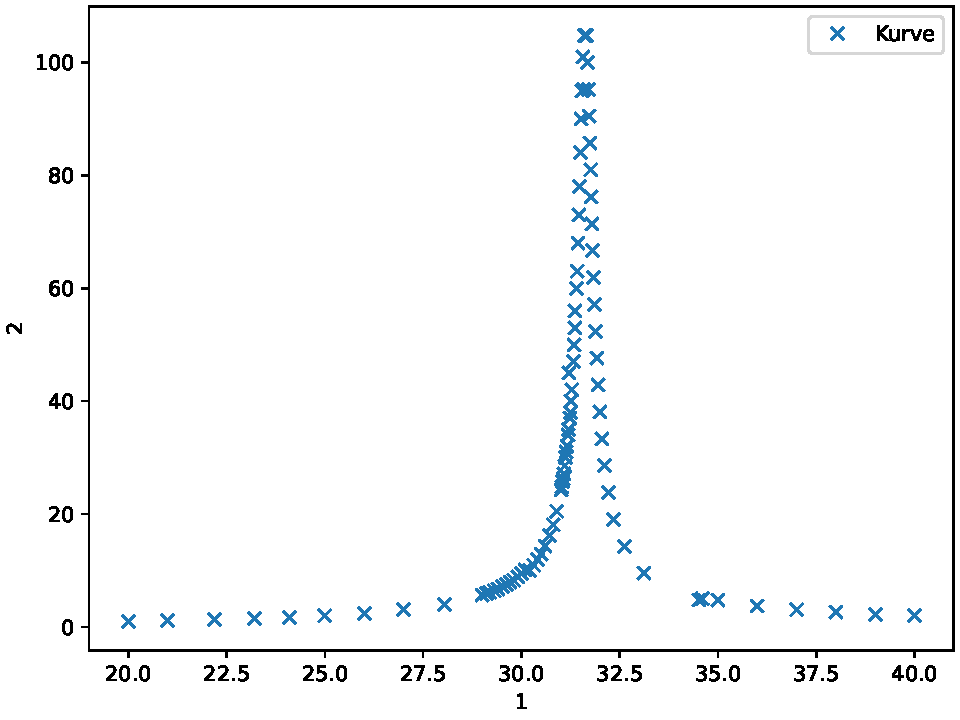
\includegraphics[height=9cm]{plot.pdf}
  \caption{Messwerte des Selektivsverstärkers mit Ausgleichskurve und Güte.}
  \label{fig:plot}
\end{figure}
Die Frequenz, bei der die maximale Ausgangsspannung erreicht ist, wird durch die Ausgleichskurve zu $\nu_0 = 31,61 \, \unit{\kilo\hertz}$ bestimmt. Die Güte wird mithilfe 
von Formel (\ref{eqn:Guete}) zu $73,52$ berechnet. 
\subsection{Theoretische Berechnung der magnetischen Suszeptibilität}
Zur Berechnung der Suszeptibilität der verschiedenen Materialien werden die Hund'schen Regeln (\ref{eqn:HundscheRegel_minus}) und (\ref{eqn:HundscheRegel_plus}) verwendet. Zur Berechnung des Landé-Faktors $g_J$ 
wird die Formel (\ref{eqn:LandeFaktor}) benutzt. Die sich ergebenden Werte für $L$, $S$, $J$ und $g_J$ 
sind in Tabelle (\ref{tab:L_S_J}) zu sehen. Die Größe $N$ wird mithilfe von 
\begin{equation}
  N = 2 \cdot \frac{\rho_w N_a}{M}
\end{equation}
berechnet. $N_a$ steht dabei für die Avogadrokonstante, $M$ für die molare Masse und $\rho_w$ für die Dichte der Probe. Der Wert der molaren Masse wird recherchiert \cite{Molare_Masse}.  
Die probenspeziefischen Werte sind in Tabelle (\ref{tab:L_S_J}) aufgelistet.

\begin{table}[H]
  \centering
  \caption{Theoriewerte für $L, S$, $J$, $g_J$, $\rho_w$, $M$ und $N$}
  \label{tab:L_S_J}
  \begin{tblr}{colspec={c c c c c c c c}}
      \toprule
      $\text{Material}$ & $L$ & $S$ & $J$ & $g_J$ & $\cdot \, 10³ \, \rho_w \,\left[ \unit[per-mode=fraction]{\kilo\gram\per\cubic\meter} \right]$ & $\cdot \, 10^{-3} \, M \, \left[ \unit[per-mode=fraction]{\kilo\gram\per\mol} \right]$ & $\cdot \, 10^{28} \, N \left[\frac{1}{\unit{\cubic\meter}}\right]$ \\
      \midrule
      \ce{Nd2O3} & 6 & 1,5 & 4,5 & 0,7272 & 7,24 & 336,5 & 2,59 \\
      \ce{Gd2O3} & 0 & 3,5 & 3,5 & 2,0000 & 7,40 & 362,5 & 2,46 \\
      \ce{Dy2O3} & 5 & 2,5 & 7,5 & 1,3333 & 7,8 & 373,0 & 2,52 \\  
      \bottomrule
  \end{tblr}
\end{table}

Die mithilfe von Formel (\ref{eqn:paramagnetische_Suszeptibilität}) berechnete Suszeptibilität ist in Tabelle (\ref{tab:chi_theo}) aufgelistet. 
\begin{table}[H]
  \centering
  \caption{Theoriewerte für $\chi_{\text{theo}}$}
  \label{tab:chi_theo}
  \begin{tblr}{colspec={c r}}
      \toprule
      $\text{Material}$ & $\cdot \, 10^{-3} \, \chi_{\text{theo}}$ \\
      \midrule
      \ce{Nd2O3} &  2,9877\\
      \ce{Gd2O3} &  13,6565\\
      \ce{Dy2O3} &  25,0409\\  
      \bottomrule
  \end{tblr}
\end{table}

\subsection{Berechnung der Suszeptibilität aus Messwerten}
Zur experimentellen Bestimmung der Suszeptibilität wird der reale Querschnitt $Q_{\text{real}}$ der Probe benötigt. Dieser wird mithilfe von Formel (\ref{eqn:Querschnitt_Real}) berechnet. 
Zur Berechnung werden die Messdaten in Tabelle (\ref{tab:Laenge_Gewicht}) verwendet. Das durch diese Werte berechnete $Q_{\text{real}}$ ist ebenfalls 
in Tabelle (\ref{tab:Laenge_Gewicht}) aufgelistet. 
\begin{table}[H]
  \centering
  \caption{Länge, Gewicht und realer Querschnitt der Proben}
  \label{tab:Laenge_Gewicht}
  \begin{tblr}{colspec={c c c c}}
      \toprule
      $\text{Material}$ & $\text{Länge} \left[\unit{\centi\meter}\right]$ & $\text{Gewicht} \left[\unit{\gram}\right]$ & $Q_{\text{real}} \left[\unit{\meter\squared}\right]$\\
      \midrule
      \ce{Nd2O3} &  15,9 & 18,48 & 1,6053 $\cdot 10^{-5}$\\
      \ce{Gd2O3} &  15,7 & 14,08 & 1,2119 $\cdot 10^{-5}$\\
      \ce{Dy2O3} &  15,8 & 14,38 & 1,1668 $\cdot 10^{-5}$\\  
      \bottomrule
  \end{tblr}
\end{table}

Die aus Messdaten bestimmte Suszeptibilität $\chi_{\text{exp,1}}$ wird mithilfe von Formel (\ref{eqn:Suszeptibilität_ersteMethode}) berechnet. Der dazu benötigte 
Querschnitt der Spule $F$ beträgt $86,6 \cdot 10^{-6} \, [\unit{\meter\squared}]$. Die gemessene Brückenspannung $U_{\text{Br}}$ und die gemessene Eingangsspannung $U_{\text{Sp}}$ sind in Tabelle (\ref{tab:Bruecken_und_Eingangsspannung}) aufgeführt.

\begin{table}[H]
  \centering
  \caption{Gemessene Brückenspannung und Eingangsspannung}
  \label{tab:Bruecken_und_Eingangsspannung}
  \begin{tblr}{colspec={c | c c c | c c c}}
      \toprule
      $\text{Material}$ & $U_{\text{Br,1}} \left[\unit{\milli\volt}\right]$ & $U_{\text{Br,2}} \left[\unit{\milli\volt}\right]$ & $U_{\text{Br,3}} \left[\unit{\milli\volt}\right]$ & $U_{\text{Sp,1}} \left[\unit{\milli\volt}\right]$ & $U_{\text{Sp,2}} \left[\unit{\milli\volt}\right]$ & $U_{\text{Sp,3}} \left[\unit{\milli\volt}\right]$\\
      \midrule
      \ce{Nd2O3} & 31 & 36 & 35 & 37 & 35 & 35\\
      \ce{Gd2O3} & 31 & 32 & 32 & 46 & 47 & 51\\
      \ce{Dy2O3} & 34 & 34 & 34 & 81 & 81 & 80\\  
      \bottomrule
  \end{tblr}
\end{table}
Die aus diesen Werten berechnete Suszeptibilität ist in Tabelle (\ref{tab:chi_exp_1}) aufgelistet.
\begin{table}[H]
  \centering
  \caption{Mithilfe der ersten Methode experimentell bestimmte Werte für $\chi_{\text{exp,1}}$}
  \label{tab:chi_exp_1}
  \begin{tblr}{colspec={c c}}
      \toprule
      $\text{Material}$ & $\chi_{\text{exp,1}}$ \\
      \midrule
      \ce{Nd2O3} &  22,60 $\pm \, 1,10$\\
      \ce{Gd2O3} &  43,30 $\pm \, 1,50$\\
      \ce{Dy2O3} &  70,43 $\pm \, 0,29$ \\  
      \bottomrule
  \end{tblr}
\end{table}
\\
Für die Bestimmung der Suszeptibilität $\chi_{\text{exp,2}}$ wird nach Formel (\ref{eqn:Suszeptibilität_zweiteMethode}) der Widerstand $R_3$ vor dem Einführen der Probe, bei dem die Spannung minimal ist, benötigt. Außerdem wird die Differenz $\Delta R$ zwischen $R_3$ und dem Widerstand $R'_3$ nach Einführen der Probe, bei dem die Spannung minimal ist, verwendet.
Es gilt: $$\Delta R = |R_3 - R'_3| \, .$$  
Diese Größen sind in Tabelle (\ref{tab:Widerstaende}) aufgeführt.
\begin{table}[H]
  \centering
  \caption{Gemessene Widerstände $R_3$, $R'_3$ und berechnete Differenz $\Delta R$  }
  \label{tab:Widerstaende}
  \begin{tblr}{colspec={r r r r}}
      \toprule
      $\text{Material}$ & $R_3 \cdot 5 \left[\unit{\milli\ohm}\right]$ &  $R'_3 \cdot 5 \left[\unit{\milli\ohm}\right]$ & $\Delta R \cdot 5 \left[\unit{\milli\ohm}\right]$ \\
      \midrule
      \ce{Nd2O3} & 547 & 517 & 30 \\
       & 544 & 539 & 5\\
       & 560 & 526 & 34\\
      \ce{Gd2O3} & 547 & 375 & 172\\
       & 548 & 382 & 166\\
       & 566 & 408 & 158\\
      \ce{Dy2O3} & 548 & 210 & 338\\
       & 547 & 239 & 308\\
       & 539 & 227 & 312\\  
      \bottomrule
  \end{tblr}
\end{table}
Die mithilfe von Formel (\ref{eqn:Suszeptibilität_zweiteMethode}) berechnete Suszeptibilität $\chi_{\text{exp,2}}$ ist in Tabelle
(\ref{tab:chi_exp_2}) aufgelistet.
\begin{table}[H]
  \centering
  \caption{Mithilfe der zweiten Methode experimentell bestimmte Werte für $\chi_{\text{exp,2}}$}
  \label{tab:chi_exp_2}
  \begin{tblr}{colspec={c c}}
      \toprule
      $\text{Material}$ & $\chi_{\text{exp,1}}$ \\
      \midrule
      \ce{Nd2O3} &  0,45 $\pm \, 0,16$ \\
      \ce{Gd2O3} &  4,27 $\pm \, 0,28$ \\
      \ce{Dy2O3} &  8,70 $\pm \, 0,23$ \\  
      \bottomrule
  \end{tblr}
\end{table}
%Siehe \autoref{fig:plot}!